% -*- root: root.tex -*-
\RequirePackage[l2tabu, orthodox]{nag}                  % Checks for obsolete syntax and package % Layout
\documentclass[11pt,a4paper,oneside]{article}

%% font
\usepackage{MnSymbol}
\usepackage[mathlf,textlf]{MinionPro}
\usepackage[T1]{fontenc}
\usepackage{enumitem}
\usepackage[utf8]{inputenc}

%% Author
\def\myaffiliation{University of Copenhagen}
\def\myauthor{Rud Faden}
\def\myemail{rud.faden@econ.ku.dk}
\def\mytitle{No cure no pay contracts with limited liability}
\def\mykeywords{Information aggregation, physician,}

%% packages
\usepackage[drafting]{faden}
\pgfplotsset{compat=1.9}
\usetikzlibrary{decorations.pathreplacing}
\graphicspath{{../fig/}}
\usepackage{commath}
\usepackage[colorinlistoftodos,draft]{todonotes}        % todo notes
\setlength{\marginparwidth}{3.5cm} % fix for todo notes


%% custom macroes 

%% biblatex path
\addbibresource{Remote.bib}

% Author and title
\title{\mytitle}
\author{
{\myauthor} \\
\textit{\small \myaffiliation} \\
\small{\texttt{\href{\myemail}{\myemail}}}
}
\date{\today} % no date

%% Version control
\immediate\write18{sh ./vc}
%%% This file has been generated by the vc bundle for TeX.
%%% Do not edit this file!
%%%
%%% Define Git specific macros.
\gdef\GITHash{9d5e3b469d5f4d8f56c54cfc33fcab676c8905ff}%
\gdef\GITAbrHash{9d5e3b4}%
\gdef\GITParentHashes{904e5d3ddc0482da848ff729ca2451b0fd5c4aee}%
\gdef\GITAbrParentHashes{904e5d3}%
\gdef\GITAuthorName{Rud Faden}%
\gdef\GITAuthorEmail{rudfaden@gmail.com}%
\gdef\GITAuthorDate{2015-04-27 11:47:18 +0200}%
\gdef\GITCommitterName{Rud Faden}%
\gdef\GITCommitterEmail{rudfaden@gmail.com}%
\gdef\GITCommitterDate{2015-04-27 11:47:18 +0200}%
%%% Define generic version control macros.
\gdef\VCRevision{\GITAbrHash}%
\gdef\VCAuthor{\GITAuthorName}%
\gdef\VCDateRAW{2015-04-27}%
\gdef\VCDateISO{2015-04-27}%
\gdef\VCDateTEX{2015/04/27}%
\gdef\VCTime{11:47:18 +0200}%
\gdef\VCModifiedText{\textcolor{red}{with local modifications!}}%
%%% Assume clean working copy.
\gdef\VCModified{0}%
\gdef\VCRevisionMod{\VCRevision}%



\begin{document}
\maketitle
\begin{abstract}
This paper examines a principal agent model in which a risk neutral physician makes an ex-ante effort choice while receiving payment from a risk neutral
principal. It is assumed that the physician is subject to limited liability, such
that he cannot be punished for bad outcome, but only rewarded for good outcomes.
\end{abstract}

\section{Model} % (fold)
\label{sec:model}
There is a risk neutral physician that cures a continuum of patients with a value to the principal of $y\in[0,\infty)$ and receives payment $R(y)$. The physician cures patient with effort $e$. I assume that the probability of curing a patient is monotonically increasing in effort (monotone likelihood ratio property), such that 
\begin{align}
    \pder{y}\left(\frac{g_e(y\mid e)}{g(y\mid e)}\right)>0 \label{eq:mlrp}
\end{align}
for all $e>0$ and $y\ge 0$. In addition I assume that $\cEX{y|e=0}=0$. Further I also assume that the distribution functions satisfies convexity of the distribution function (CDFC).\footnote{The CDFC assumption implies that $\pder[G(y|e)][2]{e}\geq0$. See \textcite[][p. 1362]{Rogerson1985FirstOrder}}

The principal observes the physicians value of cured patients ex-ante. Therefore the hospital specifies a contract that pays the physician $R(y)$.

Further it is assumed that the payoff is bounded by limited liability. This implies that (i) the principal cannot be required to pay the physician more than the value of the production, and (ii) the physician cannot be required to make payments to the hospital.  Therefore the payment function is bounded by $0\leq R(y)\leq y$.

Let $U(y,e)$ denote the physicians continuous and twice differential utility function given by 

\begin{align}
    U(R,e)=\int_0^\infty R(y)g(y|e)\dif y-C(e) \label{eq:utility}
\end{align}

and the principals payoff is given by 
\begin{align}
    V(y,R(y))=\int_0^\infty (y-R(y))g(y|e)\dif y
\end{align}
\section{Optimal payment with a risk neutral agent} % (fold)
\label{sec:optimal_payment_with_a_risk_neutral_agent}


Unfortunately neither existence or uniqueness of a solution to \cref{eq:utility} can be guaranteed. To reduce the ambiguity I follow~\textcite{Innes1990Limited} and introduce the first assumption.

\begin{assumption}{[\textcite{Innes1990Limited}]}
\label{asump:effort}
 There exists a finite $e_{\max}$ such that 
\[
    \lim_{e \rightarrow e_{\max}} \cEX*{U(y,e)|e}<\cEX*{U(y,0)|0}
\]
 \end{assumption}

 \Cref{asump:effort} indicates that there is some disutility to effort and that this effort is increases as $e\rightarrow e_{\max}$. Therefore the physicians effort choice can be limited to $\left[0,e_{\max}\right]$

\begin{lemma}{[\textcite{Innes1990Limited}]}
\label{lem:bounded}
For all $R(y)$ functions satisfying limited liability $0\leq R(y)\leq y$, (i) $\cEX*{U(y,e)|e}$ is bounded from above and below on the domain $e\in\left[0,e_{\max}\right]$, and therefore there exists at least one solution to \cref{eq:utility}
\end{lemma} 

\begin{proof}
For all $R(y)$ satisfying the limited liability constraint $\cEX{U(y,e)|e}\geq\cEX{U(R(y),e)|e}$, and for $e\in\left[0,e_{\max}\right]$, $\cEX{U(R(y),e)|e}\allowbreak\geq\cEX{U(0,e)|e}\allowbreak\geq\cEX{U(R(y)-k^*,e)|e}$, $k^*=\cEX{R(y)|e_{\max}}$. Since $\cEX{U(R(y),e)|e}$ and thereby also $\cEX{U(R(y)-k^*,e)|e}$ is continuous on the compact set $e\in\left[0,e_{\max}\right]$, implying result (i). Result (ii) then follows from the extreme value theorem.
\end{proof}

\Cref{lem:bounded} implies that there exists an optimal level of effort given a eligible payoff function.

Given \cref{eq:utility} and a fixed payment function $R(y)$, the physician will choose effort to solve the following problem
\begin{subequations}
\label{eq:khun-tucker}
\begin{align}
    \max_{R,e} & \int_0^{\infty}R(y)g(y|e)\dif y-C(e)\label{subeq:khun-tucker1} \\
    \text{s.t. }    & \int_{0}^{\infty} (y-R(y))g(y|e)\dif y\geq y_L^0 \label{subeq:khun-tucker2} \\
                    & \cEX{U(R,e)|e}\leq \cEX{U(R,e^*)|e} \label{subeq:khun-tucker3}\\
                    & 0\leq R(y)\leq y \label{subeq:khun-tucker4}
\end{align}
\end{subequations}
To find a solution to \cref{eq:khun-tucker} is difficult and few general results can obtained. To make the problem more tractable incentive comparability constraint in \cref{subeq:khun-tucker3} is often replaced by the first order derivative.\footnote{This approach is in general only valid when the agent is risk neutral. In \cref{sec:optimal_payment_with_a_risk_averse_agent} I will solve the problem when the agent is risk averse}
\begin{proposition}
\label{prop:payment-function}
If $R$ solves the maximization problem in \cref{subeq:khun-tucker1}, then there is some threshold value $y^*$, such that 

\[
    R^*(y)=\begin{cases}
                0 & \text{for } y< y^* \\
                y & \text{for } y\geq y^*
            \end{cases}            
\]
\end{proposition}

\begin{proof}
Replacing \cref{subeq:khun-tucker3} with it's (relaxed) first order condition, and writing down the Lagrangian I get that 
\begin{align}
    \mathcal{L}=R(y)g(y|e)-C(e)+\mu [R(y)g_e(y|e)-C_e(e)]+\lambda [(y-R(y))g(y|e)-y_L^0]
\end{align}
which can also be written as 
\begin{equation}
\begin{split}
   R(y)\left[g(y|e)+\mu g_(y|e)\right]+(y-R(y))\lambda g(y|e)+ \\
                         & yg(y|e)-\mu C_e(e)-\lambda y_L^0 \label{eq:lagrange}
\end{split}
\end{equation}

Only the first to terms of \cref{eq:lagrange} depends on the size of $R(y)$ and thereby determines the maximum. If the first term is larger than the second term

\begin{align}
     R(y)\left[g(y|e)+\mu g_(y|e)\right]>(y-R(y))\lambda g(y|e) \label{eq:max-payment}
\end{align}

the whole expression is increasing in $R(y)$, therefore $R(y)$ should be set to it's maximum $R(y)=y$. If the opposite is true 
\begin{align}
     R(y)\left[g(y|e)+\mu g_(y|e)\right]<(y-R(y))\lambda g(y|e) \label{eq:min-payment}
\end{align}
the expression is decreasing in $R$, and $R(y)$ should be set to it's minimum $R(y)=0$. Note that \cref{eq:min-payment} can be written as

\begin{align}
   1+\mu \frac{g_e(y|e)}{g(y|e)}<\lambda \label{eq:min-payment-2}
\end{align}

Given \cref{eq:mlrp}, the left hand side of \cref{eq:min-payment-2} is increasing in $y$ this inequality is satisfied for some $y$ below a threshold level $y^*$. Above $y^*$ \cref{eq:max-payment} holds. Thereby the payment function is 0 for some $y<y^*$ and $y$ for some level above $y> y^*$ as stated in \cref{prop:payment-function}.
% \footnote{Alternatively, solving the Lagrangian I get that 
% \[
%     R \left( y \right) =-\left(1+\lambda \right){\frac {y_{L}}{\mu\,g_{
% e} \left( y|e \right) }}+y
% \]
% which is negative for ${\left( 1+\lambda \right)\frac {y_{L}}{\mu\,g_{
% e} \left( y|e \right) }}>y$. Therefore $R(y)=0$ by \cref{subeq:khun-tucker4}. But note that  $g_e(y|e)$ is increasing in $y$, such that $ \left( 1+\lambda \right){\frac { y_{L}}{\mu\,g_{e} \left( y|e \right) }}$ goes to zero as $y$ increases. So there must be some $y$ for which $R(y)=y$ 
% }
What remains is to show that the solution to \cref{eq:khun-tucker} is in fact an optimum. Following \textcite{Rogerson1985FirstOrder} it is sufficient to show that $\mu>0$. If $\mu\leq0$, payment is non-increasing in output. By \cref{asump:effort} the physician therefore chooses $e=0$. However, $e=0$ is not feasible because of the assumption that $\cEX{y|e=0}=0$ and condition \cref{subeq:khun-tucker2}. Therefore for $e>0$, $\mu$ must be positive. 
\end{proof}

\begin{figure}[htbp]
    \centering
    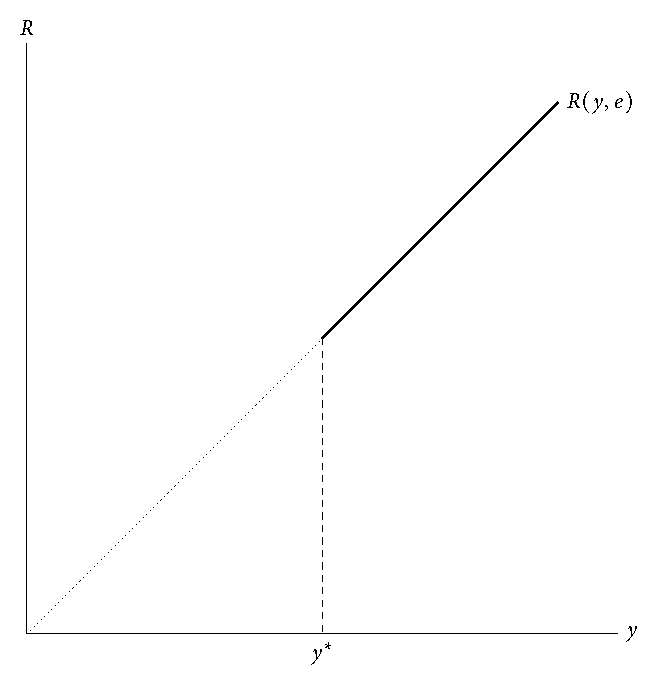
\includegraphics[width=0.95\textwidth]{optimal-R.pdf}
    \caption{The payment function $R(y)$. Before $y^*$ the physician is payed nothing and after $y^*$ the physician is the payed maximum of $R(y)$ }
    \label{fig:label}
\end{figure}

\subsection{An alternative proof} % (fold)
\label{sub:an_alternative_proof}
Give \cref{eq:khun-tucker}  Lagrangian is
\begin{align}
    \begin{split}
        \mathcal{L}=R(y)g(y|e)-C(e)+\mu [R(y)g_e(y|e)-C_e(e)]+ \\ 
        \lambda [(y-R(y))g(y|e)-y_L^0]+\theta(y) R(y)+\theta(y)\left(y-R(y)\right)
    \end{split}
\end{align}
The first order conditions are
\begin{subequations}
\label{eq:foc}
\begin{align}
    g(y|e)\left[1-\lambda+\mu \frac{g_e(y|e)}{g(y|e)}\right]+\theta(y)-\eta(y) \label{eq:foc1} \\
    R(y)\left[(1-\lambda)g_e(y|e)+\mu g_{ee}(y|e)\right]-C_{ee}(e)
\end{align}
\end{subequations}
Because of nonnegativity and complementary slackness conditions for $\theta(y)$ and $\eta(y)$, \cref{eq:foc1} yields
\begin{subequations}
\label{eq:KT-analysis}
\begin{alignat}{3}
\phi(y,e) = g(y|e)\left[1-\lambda+\mu \frac{g_e(y|e)}{g(y|e)}\right]
   & \: > \: & 0 &\enspace \Rightarrow &&\enspace R(y)=y \label{subeq:large-y}\\
 \phi(y,e)   & \: = \: & 0 &\enspace \Rightarrow &&\enspace R(y)\in [0,y] \label{subeq:interval-y} \\
 \phi(y,e)   & \: < \: & 0 &\enspace \Rightarrow &&\enspace R(y) =0 \label{subeq:small-y}
\end{alignat}
\end{subequations}

It is clear from \cref{eq:foc1,eq:mlrp} that for $y$ large enough \cref{subeq:large-y} is always feasible. However, feasibility of \cref{subeq:interval-y,subeq:large-y} is not guaranteed, even for $y=0$



% paragraph case_1_lambda_0_ (end)
% subsection an_alternative_proof (end)
% section optimal_payment_with_a_risk_neutral_agent (end)
\section{Optimal payment with a risk averse agent} % (fold)
\label{sec:optimal_payment_with_a_risk_averse_agent}
% However, this approach have been shown to be invalid in general. \textcite{Rogerson1985FirstOrder}, however, has showed that replacing \cref{subeq:khun-tucker3} with 
% \[
%     \pder{e}R(y)g(y|e)-C(e)\geq0
% \]
% section optimal_payment_with_a_risk_averse_agent (end)
% section model (end)
\printbibliography%
\end{document}